\documentclass[]{book}
\usepackage{lmodern}
\usepackage{amssymb,amsmath}
\usepackage{ifxetex,ifluatex}
\usepackage{fixltx2e} % provides \textsubscript
\ifnum 0\ifxetex 1\fi\ifluatex 1\fi=0 % if pdftex
  \usepackage[T1]{fontenc}
  \usepackage[utf8]{inputenc}
\else % if luatex or xelatex
  \ifxetex
    \usepackage{mathspec}
  \else
    \usepackage{fontspec}
  \fi
  \defaultfontfeatures{Ligatures=TeX,Scale=MatchLowercase}
    \setmainfont[]{Open Sans}
\fi
% use upquote if available, for straight quotes in verbatim environments
\IfFileExists{upquote.sty}{\usepackage{upquote}}{}
% use microtype if available
\IfFileExists{microtype.sty}{%
\usepackage{microtype}
\UseMicrotypeSet[protrusion]{basicmath} % disable protrusion for tt fonts
}{}
\usepackage[margin=1in]{geometry}
\usepackage{hyperref}
\hypersetup{unicode=true,
            pdftitle={Визуализация и анализ географических данных на языке R},
            pdfauthor={Тимофей Самсонов},
            pdfborder={0 0 0},
            breaklinks=true}
\urlstyle{same}  % don't use monospace font for urls
\usepackage{natbib}
\bibliographystyle{apalike}
\usepackage{color}
\usepackage{fancyvrb}
\newcommand{\VerbBar}{|}
\newcommand{\VERB}{\Verb[commandchars=\\\{\}]}
\DefineVerbatimEnvironment{Highlighting}{Verbatim}{commandchars=\\\{\}}
% Add ',fontsize=\small' for more characters per line
\usepackage{framed}
\definecolor{shadecolor}{RGB}{248,248,248}
\newenvironment{Shaded}{\begin{snugshade}}{\end{snugshade}}
\newcommand{\KeywordTok}[1]{\textcolor[rgb]{0.13,0.29,0.53}{\textbf{#1}}}
\newcommand{\DataTypeTok}[1]{\textcolor[rgb]{0.13,0.29,0.53}{#1}}
\newcommand{\DecValTok}[1]{\textcolor[rgb]{0.00,0.00,0.81}{#1}}
\newcommand{\BaseNTok}[1]{\textcolor[rgb]{0.00,0.00,0.81}{#1}}
\newcommand{\FloatTok}[1]{\textcolor[rgb]{0.00,0.00,0.81}{#1}}
\newcommand{\ConstantTok}[1]{\textcolor[rgb]{0.00,0.00,0.00}{#1}}
\newcommand{\CharTok}[1]{\textcolor[rgb]{0.31,0.60,0.02}{#1}}
\newcommand{\SpecialCharTok}[1]{\textcolor[rgb]{0.00,0.00,0.00}{#1}}
\newcommand{\StringTok}[1]{\textcolor[rgb]{0.31,0.60,0.02}{#1}}
\newcommand{\VerbatimStringTok}[1]{\textcolor[rgb]{0.31,0.60,0.02}{#1}}
\newcommand{\SpecialStringTok}[1]{\textcolor[rgb]{0.31,0.60,0.02}{#1}}
\newcommand{\ImportTok}[1]{#1}
\newcommand{\CommentTok}[1]{\textcolor[rgb]{0.56,0.35,0.01}{\textit{#1}}}
\newcommand{\DocumentationTok}[1]{\textcolor[rgb]{0.56,0.35,0.01}{\textbf{\textit{#1}}}}
\newcommand{\AnnotationTok}[1]{\textcolor[rgb]{0.56,0.35,0.01}{\textbf{\textit{#1}}}}
\newcommand{\CommentVarTok}[1]{\textcolor[rgb]{0.56,0.35,0.01}{\textbf{\textit{#1}}}}
\newcommand{\OtherTok}[1]{\textcolor[rgb]{0.56,0.35,0.01}{#1}}
\newcommand{\FunctionTok}[1]{\textcolor[rgb]{0.00,0.00,0.00}{#1}}
\newcommand{\VariableTok}[1]{\textcolor[rgb]{0.00,0.00,0.00}{#1}}
\newcommand{\ControlFlowTok}[1]{\textcolor[rgb]{0.13,0.29,0.53}{\textbf{#1}}}
\newcommand{\OperatorTok}[1]{\textcolor[rgb]{0.81,0.36,0.00}{\textbf{#1}}}
\newcommand{\BuiltInTok}[1]{#1}
\newcommand{\ExtensionTok}[1]{#1}
\newcommand{\PreprocessorTok}[1]{\textcolor[rgb]{0.56,0.35,0.01}{\textit{#1}}}
\newcommand{\AttributeTok}[1]{\textcolor[rgb]{0.77,0.63,0.00}{#1}}
\newcommand{\RegionMarkerTok}[1]{#1}
\newcommand{\InformationTok}[1]{\textcolor[rgb]{0.56,0.35,0.01}{\textbf{\textit{#1}}}}
\newcommand{\WarningTok}[1]{\textcolor[rgb]{0.56,0.35,0.01}{\textbf{\textit{#1}}}}
\newcommand{\AlertTok}[1]{\textcolor[rgb]{0.94,0.16,0.16}{#1}}
\newcommand{\ErrorTok}[1]{\textcolor[rgb]{0.64,0.00,0.00}{\textbf{#1}}}
\newcommand{\NormalTok}[1]{#1}
\usepackage{longtable,booktabs}
\usepackage{graphicx,grffile}
\makeatletter
\def\maxwidth{\ifdim\Gin@nat@width>\linewidth\linewidth\else\Gin@nat@width\fi}
\def\maxheight{\ifdim\Gin@nat@height>\textheight\textheight\else\Gin@nat@height\fi}
\makeatother
% Scale images if necessary, so that they will not overflow the page
% margins by default, and it is still possible to overwrite the defaults
% using explicit options in \includegraphics[width, height, ...]{}
\setkeys{Gin}{width=\maxwidth,height=\maxheight,keepaspectratio}
\IfFileExists{parskip.sty}{%
\usepackage{parskip}
}{% else
\setlength{\parindent}{0pt}
\setlength{\parskip}{6pt plus 2pt minus 1pt}
}
\setlength{\emergencystretch}{3em}  % prevent overfull lines
\providecommand{\tightlist}{%
  \setlength{\itemsep}{0pt}\setlength{\parskip}{0pt}}
\setcounter{secnumdepth}{5}
% Redefines (sub)paragraphs to behave more like sections
\ifx\paragraph\undefined\else
\let\oldparagraph\paragraph
\renewcommand{\paragraph}[1]{\oldparagraph{#1}\mbox{}}
\fi
\ifx\subparagraph\undefined\else
\let\oldsubparagraph\subparagraph
\renewcommand{\subparagraph}[1]{\oldsubparagraph{#1}\mbox{}}
\fi

%%% Use protect on footnotes to avoid problems with footnotes in titles
\let\rmarkdownfootnote\footnote%
\def\footnote{\protect\rmarkdownfootnote}

%%% Change title format to be more compact
\usepackage{titling}

% Create subtitle command for use in maketitle
\newcommand{\subtitle}[1]{
  \posttitle{
    \begin{center}\large#1\end{center}
    }
}

\setlength{\droptitle}{-2em}
  \title{Визуализация и анализ географических данных на языке R}
  \pretitle{\vspace{\droptitle}\centering\huge}
  \posttitle{\par}
  \author{Тимофей Самсонов}
  \preauthor{\centering\large\emph}
  \postauthor{\par}
  \predate{\centering\large\emph}
  \postdate{\par}
  \date{2017-09-21}

\usepackage{booktabs}
\usepackage{amsthm}
\makeatletter
\def\thm@space@setup{%
  \thm@preskip=8pt plus 2pt minus 4pt
  \thm@postskip=\thm@preskip
}
\makeatother

\begin{document}
\maketitle

{
\setcounter{tocdepth}{1}
\tableofcontents
}
\chapter*{Введение}
\addcontentsline{toc}{chapter}{Введение}

Добро пожаловать в курс ``Визуализация и анализ географических данных на
языке R''! В данном курсе мы освоим азы программирования на языке R, а
затем научимся использовать его для решения географических задач.
Никаких предварительных знаний и навыков программирования не требуется.

Для успешного прохождения курса на вашем компьютере должно быть
установлено следующее программное обеспечение:

\begin{itemize}
\tightlist
\item
  Язык \href{https://cran.r-project.org}{R}
\item
  Среда разработки
  \href{https://www.rstudio.com/products/rstudio/download3/}{RStudio}
\end{itemize}

Выбирайте инсталлятор, соответствующий вашей операционной системе.
Обратите внимание на то, что RStudio не будет работать, пока вы не
установите базовые библиотеки языка R. Поэтому обе вышеуказанные
компоненты ПО обязательны для установки.

\section*{Форматы представления материалов}\label{--}
\addcontentsline{toc}{section}{Форматы представления материалов}

Прадлагаемый вашему вниманию курс состоит из ряда лекций (модулей),
каждый из которых представлен в двух форматах: \textbf{HTML} и
\textbf{R}.

\subsection*{Файл HTML}\label{-html}
\addcontentsline{toc}{subsection}{Файл HTML}

Файл \textbf{HTML} доступен в каждом модуле под названием \emph{Лекция
1}, \emph{Лекция 2} и т.д. Его удобно использовать в качестве
справочника при выполнении заданий и подготовки к занятиям. Помимо
текста и специальным образом форматированных фрагментов исходного кода,
он содержит результаты генерации графиков и карт, а также навигацию по
разделам.

Фрагменты исходного кода в тексте выглядят следующим образом:

\begin{Shaded}
\begin{Highlighting}[]
\NormalTok{a <-}\StringTok{ }\DecValTok{5}
\KeywordTok{sin}\NormalTok{(}\KeywordTok{sqrt}\NormalTok{(a))}
\NormalTok{## [1] 0.7867491}
\KeywordTok{sqrt}\NormalTok{(}\KeywordTok{sin}\NormalTok{(a) }\OperatorTok{+}\StringTok{ }\DecValTok{2}\NormalTok{)}
\NormalTok{## [1] 1.020331}
\end{Highlighting}
\end{Shaded}

Обычным шрифтом \texttt{sin(sqrt(a))} в этих фрагментах показан исходный
код, а бледным курсивом \emph{\texttt{\#\#\ {[}1{]}\ 0.7867491}} ---
результат выполнения этого кода, который выводится в консоль среды
разработки (в нашем случае это RStudio).

\begin{quote}
Если вы хотите сохранить файл HTML себе и просматривать локально,
достаточно после его открытия щелкнуть внутри страницы в любом месте
правой кнопкой мыши (сокращенно ПКМ) и выбрать команду \emph{Сохранить},
\emph{Сохранить как} или \emph{Сохранить фрейм как} (в зависимости от
браузера формулировка может меняться).
\end{quote}

\subsection*{Файл R}\label{-r}
\addcontentsline{toc}{subsection}{Файл R}

Файл \textbf{R} доступен в каждом модуле под названием \emph{Исходный
код лекции 1}, \emph{Исходный код лекции 2} и так далее. Файл \textbf{R}
также можно использовать при подготовке к лекциям и выполнении заданий.
Содержание файла исходного кода полностью соответствует лекции. Отличие
заключается в том, что файл \textbf{R} - это полноценно работающий
скрипт. Все команды, приведенные в лекции, можно последовательно
выполнить, а не только посмотреть на них, как это представлено в версии
\textbf{HTML}. Исходный текст лекции в файле R преобразован в
комментарии, так что вы можете последовательно читать и выполнять
команды.

Весьма полезно также \emph{создать копию} файла \textbf{R} и в процессе
знакомства с новой темой попробовать поменять различные параметры и
входные данные, чтобы посмотреть как меняется результат. В любом случае,
даже если вы что-то испортите, исходный файл всегда доступен через
систему электронного обучения, в которой вы в настоящий момент
находитесь.

\begin{quote}
Пользователи операционной системы Windows должны скачивать себе файл с
суффиксом \emph{CP1251} в названии, а OS X --- с суффиксом \emph{UTF8}.
Отличие связано с тем, что в данных операционных системах используются
разные кодировки для представления символов (текста). Если у вас при
открытии файла отображаются кракозябры или знаки вопросов --- это
значит, что кодировка файла не соответствует вашей операционной системе
или стандартным установкам RStudio. Проблему можно решить, скачав файл в
нужной кодировке или воспользовавшись командой меню \emph{File}
\textgreater{} \emph{Open With Encoding\ldots{}}
\end{quote}

\section*{Как работать с кодом}\label{---}
\addcontentsline{toc}{section}{Как работать с кодом}

Существует несколько способов выполнения исходного кода:

\begin{itemize}
\tightlist
\item
  \textbf{Выполнить одну строку}: поставить курсор в любую строку и
  нажать над редактором кода кнопку \emph{Run} или сочетание клавиш
  \texttt{Ctrl}+\texttt{Enter} (\texttt{Cmd}+\texttt{Enter} для OS X).
\item
  \textbf{Выполнить несколько строк}: выделить необходимые строки и
  нажать над редактором кода кнопку \emph{Run} или сочетание клавиш
  \texttt{Ctrl}+\texttt{Enter} (\texttt{Cmd}+\texttt{Enter} для OS X).
\item
  \textbf{Выполнить весь код} можно сразу тремя способами:

  \begin{itemize}
  \item
    Выделить весь текст и нажать над редактором кода кнопку \emph{Run}
    или сочетание клавиш \texttt{Ctrl+Enter}
    (\texttt{Cmd}+\texttt{Enter} для OS X)
  \item
    Нажать клавиатурное сочетание
    \texttt{Ctrl}+\texttt{Alt}+\texttt{Enter}
    (\texttt{Cmd}+\texttt{Alt}+\texttt{Enter} для OS X)
  \item
    Нажать в правом верхнем углу редактора кода кнопку \emph{Source}

    \begin{quote}
    Команды \emph{Source} и \texttt{Ctrl}+\texttt{Alt}+\texttt{Enter}
    могут не сработать, если у вас не установлена рабочая директория,
    или если в пути к рабочей директории содержатся кириллические
    символы (не актуально для Windows 10+ и OS X, которые являются
    системами, основанными на кодировке Unicode).
    \end{quote}
  \end{itemize}
\end{itemize}

Существует также ряд дополнительных опций выполнения кода, которые вы
можете найти в меню \emph{Code \textgreater{} Run Region}

\begin{quote}
Выполняя код построчно, делайте это последовательно, начиная с первой
строки программы. Одна из самых распространенных ошибок новичков
заключается в попытке выполнить некую строку, не выполнив
\emph{предыдущий код}. Нет никаких гарантий, что что-то получится, если
открыть файл, поставить курсор в произвольную строку посередине
программы и попытаться выполнить ее. Возможно, вам и повезет --- если
эта строка никак не зависит от предыдущего кода. Однако в реальных
программах такие строки составляют лишь небольшую долю от общего объема.
Как правило, в них происходит инициализация новых переменных стартовыми
значениями.
\end{quote}

\section*{Комментарии}
\addcontentsline{toc}{section}{Комментарии}

\textbf{Комментарии} --- это фрагменты текста программы, начинающиеся с
символа \texttt{\#}. Комментарии не воспринимаются как исполняемый код и
служат для документирования программы. При выполнении программы
содержимое комментария в зависимости от настроек среды может выводиться
или не выводиться в консоль, однако их содержание никак не влияет на
результаты выполнения программы.

\begin{quote}
Всегда пишите комментарии, чтобы по прошествии времени можно было
открыть файл и быстро восстановить в памяти логику программы и смысл
отдельных операций. Комментарии особенно необходимы, если вашей
программой будет пользоваться кто-то другой --- без них будет трудно
разобраться в программном коде.
\end{quote}

Действие комментария продолжается от символа \texttt{\#} до конца
строки. Соответственно, вы можете поставить данный символ в самом начале
строки и тогда комментарий будет занимать всю строку. Комментарий также
можно расположить справа от исполняемого кода, и тогда он будет занимать
только часть строки.

\begin{quote}
Прервать комментарий и написать справа от него исполняемый код нельзя
\end{quote}

Полнострочные комментарии часто используются для выделения разделов в
программе и написания объемных пояснений. Часто в них вводят имитации
разделительных линий с помощью символов дефиса (\texttt{-}) или
подчеркивания (\texttt{\_}), а заголовки набирают прописными буквами.
Короткие комментарии справа от фрагментов кода обычно служат пояснением
конкретных простых операций. Подобная логика употребления комментариев
не является обязательной. Вы можете оформлять их на свое усмотрение.
Главное, чтобы они выполняли свою основную функцию --- пояснять смысл
выполняемых действий. Например:

\begin{Shaded}
\begin{Highlighting}[]
\CommentTok{# ОПЕРАЦИИ С ЧИСЛАМИ}
\CommentTok{# ---------------------------}
\CommentTok{# В данном разделе рассматриваются арифметические операции, такие как сложение, вычитание, деление, деление с остатком, взятие остатка и возведение в степень:}

\NormalTok{a <-}\StringTok{ }\DecValTok{3} \OperatorTok{+}\StringTok{ }\DecValTok{2} \CommentTok{# Сложение}
\NormalTok{b <-}\StringTok{ }\DecValTok{4} \OperatorTok{^}\StringTok{ }\DecValTok{8} \CommentTok{# Возведение в степень}
\NormalTok{c <-}\StringTok{ }\NormalTok{b }\OperatorTok\StringTok{ }\NormalTok{a }\CommentTok{# Взятие остатка}

\CommentTok{# Деление}
\NormalTok{d <-}\StringTok{ }\NormalTok{c }\OperatorTok{/}\StringTok{ }\NormalTok{a }

\CommentTok{# Умножение}
\NormalTok{e <-}\StringTok{ }\NormalTok{d }\OperatorTok{*}\StringTok{ }\NormalTok{b}
\end{Highlighting}
\end{Shaded}

Однако, усердствовать с комментированием каждой мелочи в программе,
разумеется, не стоит. Со временем у вас выработается взвешенный подход к
документированию программ и понимание того, какие ее фрагменты требуют
пояснения, а какие самоочевидны.

\begin{quote}
Для быстрой вставки комментария, обозначающего новый раздел программы,
воспользуйтесь командой меню \emph{Code \textgreater{} Insert Section}
или клавиатурным сочетанием \texttt{Ctrl}+\texttt{Shift}+\texttt{R}
(\texttt{Cmd}+\texttt{Shift}+\texttt{R} для OS X)
\end{quote}

\section*{Стандарт оформления кода на R}\label{----r}
\addcontentsline{toc}{section}{Стандарт оформления кода на R}

Очень важно сразу же приучить себя грамотно, структурированно и красиво
оформлять код на языке R. Это существенно облегчит чтение и понимание
ваших программ не только вами, но и другими пользователями и
разработчиками. Помимо вышеуказанных рекомендаций по написанию
комментариев существует также определенное количество хорошо
зарекомендовавших себя и широко используемых практик оформления кода.
Эти практики есть в каждом языке программирования и их можно найти в
литературе (и в Интернете) в виде негласных сводов правил (\emph{style
guides})

Если вы не хотите быть белой вороной в мире R, вам будет полезно
внимательно ознакомиться со
\href{https://google.github.io/styleguide/Rguide.xml\#filenames}{стандартом
оформления кода на R от компании Google}, которая широко использует этот
язык в своей работе.

\begin{quote}
Стандарт оформления кода иногда также называют стилем программирования.
Мы не будем использовать этот термин, поскольку под стилем
программирования традиционно также понимают фундаментальный подход
(\emph{парадигму}) к построению программ: процедурный, функциональный,
логический, объектно-ориентированный и некоторые
\href{https://ru.wikipedia.org/wiki/Парадигма_программирования}{другие}.
\end{quote}

\section*{Названия специальных символов}\label{--}
\addcontentsline{toc}{section}{Названия специальных символов}

В \textbf{R}, как и во многих других языках программирования испльзуются
различные специальные символы. Их смысл и значение мы узнаем по ходу
изучения языка, а пока что выучите их названия, чтобы грамотно
употреблять в своей речи

\begin{longtable}[]{@{}ll@{}}
\toprule
Символ & Название\tabularnewline
\midrule
\endhead
\texttt{\$} & доллар\tabularnewline
\texttt{\#} & шарп\tabularnewline
\texttt{\&} & амперсанд\tabularnewline
\texttt{/} & прямой слэш\tabularnewline
\texttt{\textbackslash{}} & обратный слэш\tabularnewline
\texttt{\textbar{}} & пайп\tabularnewline
\texttt{\^{}} & циркумфлекс\tabularnewline
\texttt{@} & эт\tabularnewline
\texttt{\textasciitilde{}} & тильда\tabularnewline
\texttt{\textquotesingle{}\textquotesingle{}} & одинарные
кавычки\tabularnewline
\texttt{""} & двойные кавычки\tabularnewline
\texttt{\textasciigrave{}\textasciigrave{}} & обратные
кавычки\tabularnewline
\bottomrule
\end{longtable}

\section*{Установка и подключение пакетов}\label{---}
\addcontentsline{toc}{section}{Установка и подключение пакетов}

Существует \href{https://cran.r-project.org/web/packages/}{множество}
дополнительных пакетов R (вы тоже можете написать свой) практически на
все случаи жизни. Как и дистрибутив R, они доступны через
\href{https://cran.r-project.org}{CRAN (Comprehensive R Archive
Network)}. Одним из таких пакетов является, например, пакет
\texttt{openxlsx}, позволяющий читать и записывать файлы в форматах
\textbf{Microsoft Excel}.

Существует два способа установки пакетов в \textbf{RStudio}.

Во-первых, вы можете сделать это в графическом интерфесе, нажав кнопку
\emph{Install} на панели \emph{Packages} (по умолчанию эта панель
расположена в нижней правой четверти окна программы). В появившемся окне
введите название пакета и нажмите \emph{Install}:

\begin{figure}
\centering
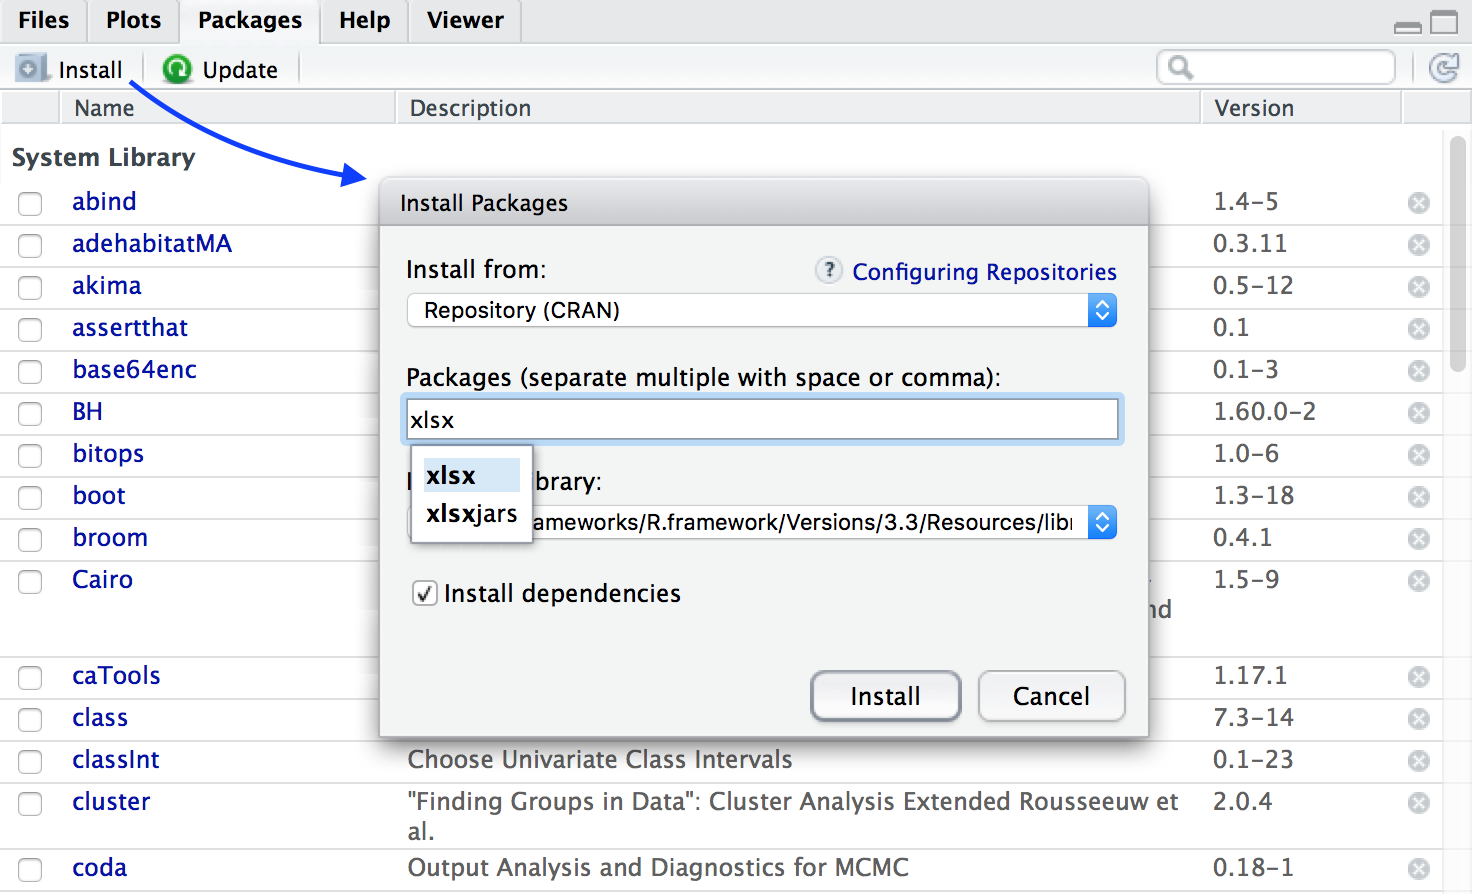
\includegraphics{images/InstallPackages.png}
\caption{\emph{Установка пакета}}
\end{figure}

Во-вторых, вы можете вызвать \emph{из консоли} команду
\texttt{install.packages()}, передав ей в качестве параметра название
пакета, заключенное в кавычки:

\begin{Shaded}
\begin{Highlighting}[]
\KeywordTok{install.packages}\NormalTok{(}\StringTok{"openxlsx"}\NormalTok{)}
\end{Highlighting}
\end{Shaded}

\begin{quote}
Внимание: никогда не включайте команду \texttt{install.packages()} в
тело скрипта. Это приведет к тому, что каждый раз при запуске программы
среда \textbf{RStudio} будет пытаться заново установить пакет, который
уже установлен. Запускайте эту функцию \emph{только из консоли}.
\end{quote}

\begin{quote}
Если по каким-то причинам вы не можете установить пакет в стандартную
системную директорию \textbf{RStudio} (например, из-за политик
безопасности, запрещающих запись в каталог \emph{Program Files} на ОС
\textbf{Windows}), то необходимо создать директорию вручную в другом
месте (куда вы имеете полный доступ) и указать ее адрес в параметре
\texttt{lib} функции \texttt{install.packages()}. Например:
\texttt{install.packages("xlsx",\ lib\ =\ "C:/Rlib/")}
\end{quote}

Подключение пакета осуществляется с помощью функции \texttt{library()},
при этом название пакета можно в кавычки не заключать:

\begin{Shaded}
\begin{Highlighting}[]
\KeywordTok{library}\NormalTok{(openxlsx)}
\end{Highlighting}
\end{Shaded}

\begin{quote}
Если пакет установлен не в стандартный каталог, а в другое место ---
например, в каталог \texttt{С:/Rlib/} (см. выше) --- то при вызове
функции \texttt{library()} необходимо указать местоположение пакета в
дополнительном параметре \texttt{lib.loc}:
\texttt{library(xlsx,\ lib.loc\ =\ "C:/Rlib")}
\end{quote}

\section*{Как ссылаться}\label{-}
\addcontentsline{toc}{section}{Как ссылаться}

Если этот курс лекций оказался полезным для вас, и вы хотите
процитировать его с списке литературы вашей работы, что ссылку можно
оформить как:

\emph{Самсонов Т.Е.} \textbf{Визуализация и анализ географических данных
на языке R.} М.: Географический факультет МГУ, 2017. DOI:
10.5281/zenodo.901911

\chapter{Атомарные типы данных}\label{data_types}

\section{Числа}\label{numbers}

Числа --- основной тип данных в R. К ним относятся \emph{числа c
плавающей точкой} и \emph{целые числа}. В терминологии R такие данные
называются \emph{интервальными}, поскольку к ним применимо понятие
интервала на числовой прямой. Целые числа относятся к \emph{дискретным
интервальным}, а числа с плавающей точкой --- к \emph{непрерывным
интервальным}. Числа можно складывать, вычитать и умножать:

\begin{Shaded}
\begin{Highlighting}[]
\DecValTok{2} \OperatorTok{+}\StringTok{ }\DecValTok{3}
\NormalTok{## [1] 5}
\DecValTok{2} \OperatorTok{-}\StringTok{ }\DecValTok{3}
\NormalTok{## [1] -1}
\DecValTok{2} \OperatorTok{*}\StringTok{ }\DecValTok{3}
\NormalTok{## [1] 6}
\end{Highlighting}
\end{Shaded}

Разделителем целой и дробной части является точка, а не запятая:

\begin{Shaded}
\begin{Highlighting}[]
\FloatTok{2.5} \OperatorTok{+}\StringTok{ }\FloatTok{3.1}
\NormalTok{## [1] 5.6}
\end{Highlighting}
\end{Shaded}

Существует также специальный оператор для возведения в степень. Для
этого вы можете использовать или двойной знак умножения (\texttt{**})
или \emph{циркумфлекс} (\texttt{\^{}}), который в обиходе называют
просто ``крышечкой'':

\begin{Shaded}
\begin{Highlighting}[]
\DecValTok{2} \OperatorTok{^}\StringTok{ }\DecValTok{3}
\NormalTok{## [1] 8}
\DecValTok{2} \OperatorTok{**}\StringTok{ }\DecValTok{3}
\NormalTok{## [1] 8}
\end{Highlighting}
\end{Shaded}

Результат деления по умолчанию имеет тип с плавающей точкой:

\begin{Shaded}
\begin{Highlighting}[]
\DecValTok{5} \OperatorTok{/}\StringTok{ }\DecValTok{3}
\NormalTok{## [1] 1.666667}
\DecValTok{5} \OperatorTok{/}\StringTok{ }\FloatTok{2.5}
\NormalTok{## [1] 2}
\end{Highlighting}
\end{Shaded}

Если вы хотите чтобы деление производилось целочисленным образом (без
дробной части) необходимо использовать оператор \texttt{\%/\%}:

\begin{Shaded}
\begin{Highlighting}[]
\DecValTok{5} \OperatorTok\StringTok{ }\DecValTok{3}
\NormalTok{## [1] 1}
\end{Highlighting}
\end{Shaded}

Остаток от деления можно получить с помощью оператора \texttt{\%\%}:

\begin{Shaded}
\begin{Highlighting}[]
\DecValTok{5} \OperatorTok\StringTok{ }\DecValTok{3}
\NormalTok{## [1] 2}
\end{Highlighting}
\end{Shaded}

Вышеприведенные арифметические операции являются бинарными, то есть
требуют наличия двух чисел. Числа называются ``операндами''. Отделять
операнды от оператора пробелом или нет --- дело вкуса. Я предпочитаю
отделять, так как это повышает читаемость кода. Следующие два выражения
эквивалентны. Однако сравните простоту их восприятия:

\begin{Shaded}
\begin{Highlighting}[]
\DecValTok{5}\OperatorTok\DecValTok{3}
\NormalTok{## [1] 1}
\end{Highlighting}
\end{Shaded}

\begin{Shaded}
\begin{Highlighting}[]
\DecValTok{5} \OperatorTok\StringTok{ }\DecValTok{3}
\NormalTok{## [1] 1}
\end{Highlighting}
\end{Shaded}

Как правило, в настоящих программах числа в явном виде встречаются лишь
иногда. Вместо этого для их обозначения используют переменные. В
вышеприведенных выражениях мы неоднократно использовали число 3. Теперь
представьте, что вы хотите проверить, каковы будут результаты, если
вместо 3 использовать 4. Вам придется заменить все тройки на четверки.
Если их много, то это будет утомительная работа, и вы наверняка что-то
пропустите. Конечно, можно использовать поиск с автозаменой, но что если
тройки надо заменить не везде? Одно и то же число может выполнять разные
функции в разных выражениях. Чтобы избежать подобных проблем, в
программе вводят переменные и присваивают им значения. Оператор
присваивания значения выглядит как \texttt{\textless{}-}

\begin{Shaded}
\begin{Highlighting}[]
\NormalTok{a <-}\StringTok{ }\DecValTok{5}
\NormalTok{b <-}\StringTok{ }\DecValTok{3}
\end{Highlighting}
\end{Shaded}

Чтобы вывести значение переменной на экран, достаточно просто ввести
его:

\begin{Shaded}
\begin{Highlighting}[]
\NormalTok{a}
\NormalTok{## [1] 5}
\NormalTok{b}
\NormalTok{## [1] 3}
\end{Highlighting}
\end{Shaded}

Мы можем выполнить над переменными все те же операции что и над
константами:

\begin{Shaded}
\begin{Highlighting}[]
\NormalTok{a }\OperatorTok{+}\StringTok{ }\NormalTok{b}
\NormalTok{## [1] 8}
\NormalTok{a }\OperatorTok{-}\StringTok{ }\NormalTok{b}
\NormalTok{## [1] 2}
\NormalTok{a }\OperatorTok{/}\StringTok{ }\NormalTok{b}
\NormalTok{## [1] 1.666667}
\NormalTok{a }\OperatorTok\StringTok{ }\NormalTok{b}
\NormalTok{## [1] 1}
\NormalTok{a }\OperatorTok\StringTok{ }\NormalTok{b}
\NormalTok{## [1] 2}
\end{Highlighting}
\end{Shaded}

Легко меняем значение второй переменной с 3 на 4 и выполняем код заново.

\begin{Shaded}
\begin{Highlighting}[]
\NormalTok{b <-}\StringTok{ }\DecValTok{4}
\NormalTok{a }\OperatorTok{+}\StringTok{ }\NormalTok{b}
\NormalTok{## [1] 9}
\NormalTok{a }\OperatorTok{-}\StringTok{ }\NormalTok{b}
\NormalTok{## [1] 1}
\NormalTok{a }\OperatorTok{/}\StringTok{ }\NormalTok{b}
\NormalTok{## [1] 1.25}
\NormalTok{a }\OperatorTok\StringTok{ }\NormalTok{b}
\NormalTok{## [1] 1}
\NormalTok{a }\OperatorTok\StringTok{ }\NormalTok{b}
\NormalTok{## [1] 1}
\end{Highlighting}
\end{Shaded}

Нам пришлось изменить значение переменной только один раз в момент ее
создания, все последующие операции остались неизменны, но их результаты
обновились!

Новую переменную можно создать на основе значений существующих
переменных:

\begin{Shaded}
\begin{Highlighting}[]
\NormalTok{c <-}\StringTok{ }\NormalTok{b}
\NormalTok{d <-}\StringTok{ }\NormalTok{a}\OperatorTok{+}\NormalTok{c}
\end{Highlighting}
\end{Shaded}

Посмотрим, что получилось:

\begin{Shaded}
\begin{Highlighting}[]
\NormalTok{c}
\NormalTok{## [1] 4}
\NormalTok{d}
\NormalTok{## [1] 9}
\end{Highlighting}
\end{Shaded}

Вы можете комбинировать переменные и заданные явным образом константы:

\begin{Shaded}
\begin{Highlighting}[]
\NormalTok{e <-}\StringTok{ }\NormalTok{d }\OperatorTok{+}\StringTok{ }\FloatTok{2.5}
\NormalTok{e}
\NormalTok{## [1] 11.5}
\end{Highlighting}
\end{Shaded}

Противоположное по знаку число получается добавлением унарного оператора
\texttt{-} перед константой или переменной:

\begin{Shaded}
\begin{Highlighting}[]
\NormalTok{f <-}\StringTok{ }\OperatorTok{-}\DecValTok{2}
\NormalTok{f}
\NormalTok{## [1] -2}
\NormalTok{f <-}\StringTok{ }\OperatorTok{-}\NormalTok{e}
\NormalTok{f}
\NormalTok{## [1] -11.5}
\end{Highlighting}
\end{Shaded}

Операция взятия остатка от деления бывает полезной, например, когда мы
хотим выяснить, является число четным или нет. Для этого достаточно
взять остаток от деления на 2. Если число является четным, остаток будет
равен нулю. В данном случае c равно 4, \texttt{d} равно 9:

\begin{Shaded}
\begin{Highlighting}[]
\NormalTok{c }\OperatorTok\StringTok{ }\DecValTok{2}
\NormalTok{## [1] 0}
\NormalTok{d }\OperatorTok\StringTok{ }\DecValTok{2}
\NormalTok{## [1] 1}
\end{Highlighting}
\end{Shaded}

\subsection{Числовые функции}\label{number_functions}

Прежде чем мы перейдем к рассмотрению прочих типов данных и структур
данных нам необходимо познакомиться с функциями, поскольку они
встречаются буквально на каждом шагу. Понятие функции идентично тому, к
чему мы привыкли в математике. Например, функция может называться
\texttt{Z}, и принимать 2 аргумента: \texttt{x} и \texttt{y}. В этом
случае она записывается как \texttt{Z(x,y)}. Чтобы получить значение
функции, необходимо подставить некоторые значения вместо \texttt{x} и
\texttt{y} в скобках. Нас даже может не интересовать, как фактически
устроена функция внутри, но важно понимать, что именно она должна
вычислять. С созданием функций мы познакомимся позднее.

Важнейшие примеры функций --- математические. Это функции взятия корня
\texttt{sqrt(x)}, модуля \texttt{abs(x)}, а также тригонометрические
функции \texttt{sin(x)}, \texttt{cos(x)}, \texttt{tan(x)} и обратные к
ним \texttt{asin(y)}, \texttt{acos(y)}, \texttt{atan(y)} и так далее. В
качестве аргумента функции можно использовать переменную, константу, а
также выражения:

\begin{Shaded}
\begin{Highlighting}[]
\KeywordTok{sqrt}\NormalTok{(a)}
\NormalTok{## [1] 2.236068}
\KeywordTok{sin}\NormalTok{(a)}
\NormalTok{## [1] -0.9589243}
\KeywordTok{tan}\NormalTok{(}\FloatTok{1.5}\NormalTok{)}
\NormalTok{## [1] 14.10142}
\KeywordTok{abs}\NormalTok{(a }\OperatorTok{+}\StringTok{ }\NormalTok{b }\OperatorTok{-}\StringTok{ }\FloatTok{2.5}\NormalTok{)}
\NormalTok{## [1] 6.5}
\end{Highlighting}
\end{Shaded}

Вы также можете легко вкладывать функции одна в одну, если результат
вычисления одной функции нужно подставить в другую:

\begin{Shaded}
\begin{Highlighting}[]
\KeywordTok{sin}\NormalTok{(}\KeywordTok{sqrt}\NormalTok{(a))}
\NormalTok{## [1] 0.7867491}
\KeywordTok{sqrt}\NormalTok{(}\KeywordTok{sin}\NormalTok{(a) }\OperatorTok{+}\StringTok{ }\DecValTok{2}\NormalTok{)}
\NormalTok{## [1] 1.020331}
\end{Highlighting}
\end{Shaded}

Также как и с арифметическими выражениями, результат вычисления функции
можно записать в переменную:

\begin{Shaded}
\begin{Highlighting}[]
\NormalTok{b <-}\StringTok{ }\KeywordTok{sin}\NormalTok{(}\KeywordTok{sqrt}\NormalTok{(a))}
\NormalTok{b}
\NormalTok{## [1] 0.7867491}
\end{Highlighting}
\end{Shaded}

Если переменной b ранее было присвоено другое значение, оно
перезапишется. Вы также можете записать в переменную результат операции,
выполненной над ней же. Например, если вы не уверены, что \texttt{a} ---
неотрицательное число, а вам это необходимо в дальнейших расчетах, вы
можете применить к нему операцию взятия модуля:

\begin{Shaded}
\begin{Highlighting}[]
\NormalTok{b <-}\StringTok{ }\KeywordTok{sin}\NormalTok{(a)}
\NormalTok{b}
\NormalTok{## [1] -0.9589243}
\NormalTok{b <-}\StringTok{ }\KeywordTok{abs}\NormalTok{(b)}
\NormalTok{b}
\NormalTok{## [1] 0.9589243}
\end{Highlighting}
\end{Shaded}

\section{Строки}\label{strings}

Строки --- также еще один важнейший тип данных. Строки состоят из
символов. Чтобы создать строковую переменную, необходимо заключить текст
строки в кавычки:

\begin{Shaded}
\begin{Highlighting}[]
\NormalTok{s <-}\StringTok{ "В историю трудно войти, но легко вляпаться (М.Жванецкий)"}
\NormalTok{s}
\NormalTok{## [1] "В историю трудно войти, но легко вляпаться (М.Жванецкий)"}
\end{Highlighting}
\end{Shaded}

Длину строки в символах можно узнать с помощью функции \texttt{nchar()}

\begin{Shaded}
\begin{Highlighting}[]
\KeywordTok{nchar}\NormalTok{(s)}
\NormalTok{## [1] 56}
\end{Highlighting}
\end{Shaded}

Строки можно складывать так же как и числа. Эта операция называется
\emph{конкатенацией}. В результате конкатенации строки состыковываются
друг с другом и получается одна строка. В отличие от чисел, конкатенация
производится не оператором \texttt{+}, а специальной функцией
\texttt{paste()}. Состыковываемые строки нужно перечислить через
запятую, их число может быть произвольно

\begin{Shaded}
\begin{Highlighting}[]
\NormalTok{s1 <-}\StringTok{ "В историю трудно войти,"}
\NormalTok{s2 <-}\StringTok{ "но легко вляпаться"}
\NormalTok{s3 <-}\StringTok{ "(М.Жванецкий)"}
\end{Highlighting}
\end{Shaded}

Посмотрим содержимое подстрок:

\begin{Shaded}
\begin{Highlighting}[]
\NormalTok{s1}
\NormalTok{## [1] "В историю трудно войти,"}
\NormalTok{s2}
\NormalTok{## [1] "но легко вляпаться"}
\NormalTok{s3}
\NormalTok{## [1] "(М.Жванецкий)"}
\end{Highlighting}
\end{Shaded}

А теперь объединим их в одну:

\begin{Shaded}
\begin{Highlighting}[]
\NormalTok{s <-}\StringTok{ }\KeywordTok{paste}\NormalTok{(s1, s2)}
\NormalTok{s}
\NormalTok{## [1] "В историю трудно войти, но легко вляпаться"}
\NormalTok{s <-}\StringTok{ }\KeywordTok{paste}\NormalTok{(s1, s2, s3)}
\NormalTok{s}
\NormalTok{## [1] "В историю трудно войти, но легко вляпаться (М.Жванецкий)"}
\end{Highlighting}
\end{Shaded}

Настоящая сила конкатенации проявляется когда вам необходимо объединить
в одной строке некоторое текстовое описание (заранее известное) и
значения переменных, которые у вас вычисляются в программе (заранее
неизвестные). Предположим, вы нашли в программе что максимальная
численность населения в Детройте пришлась на 1950 год и составила 1850
тыс. человек. Найденный год записан у вас в переменную \texttt{year}, а
население в переменную \texttt{pop}. Вы их значения пока что не знаете,
они вычислены по табличным данным в программе. Как вывести эту
информацию на экран ``человеческим''" образом? Для этого нужно
использовать конкатенацию строк.

Условно запишем значения переменных, как будто мы их знаем

\begin{Shaded}
\begin{Highlighting}[]
\NormalTok{year <-}\StringTok{ }\DecValTok{1950}
\NormalTok{pop <-}\StringTok{ }\DecValTok{1850}
\end{Highlighting}
\end{Shaded}

\begin{Shaded}
\begin{Highlighting}[]
\NormalTok{s1 <-}\StringTok{ "Максимальная численность населения в Детройте пришлась на"}
\NormalTok{s2 <-}\StringTok{ "год и составила"}
\NormalTok{s3 <-}\StringTok{ "тыс. чел"}
\NormalTok{s <-}\StringTok{ }\KeywordTok{paste}\NormalTok{(s1, year, s2, pop, s3)}
\NormalTok{s}
\NormalTok{## [1] "Максимальная численность населения в Детройте пришлась на 1950 год и составила 1850 тыс. чел"}
\end{Highlighting}
\end{Shaded}

Обратите внимание на то что мы конкатенировали строки с числами.
Конвертация типов осуществилась автоматически. Помимо этого, функция
сама вставила пробелы между строками.

\section{Даты}\label{dates}

Даты являются необходимыми при работе с временными данными. В
географическом анализе подобные задачи возникают сплошь и рядом.
Точность указания времени может быть самой различной. От года до долей
секунды. Чаще всего используются даты, указанные с точностью до дня. Для
создания даты используется функция \texttt{as.Date()}. В данном случае
точка --- это лишь часть названия функции, а не какой-то особый
оператор. В качестве аргумента функции необходимо задать дату,
записанную в виде строки. Запишем дату рождения автора (можете заменить
ее на свою):

\begin{Shaded}
\begin{Highlighting}[]
\NormalTok{birth <-}\StringTok{ }\KeywordTok{as.Date}\NormalTok{(}\StringTok{'1986/02/18'}\NormalTok{)}
\NormalTok{birth}
\NormalTok{## [1] "1986-02-18"}
\end{Highlighting}
\end{Shaded}

Сегодняшнюю дату вы можете узнать с помощью специальной функции
\texttt{Sys.Date()}:

\begin{Shaded}
\begin{Highlighting}[]
\NormalTok{current <-}\StringTok{ }\KeywordTok{Sys.Date}\NormalTok{()}
\NormalTok{current}
\NormalTok{## [1] "2017-09-21"}
\end{Highlighting}
\end{Shaded}

Даты также можно складывать и вычитать. В зависимости от дискретности
данных, вы получите результат в часах, днях, годах и т.д. Например,
узнать продолжительность жизни в днях можно так:

\begin{Shaded}
\begin{Highlighting}[]
\NormalTok{livedays <-}\StringTok{ }\NormalTok{current }\OperatorTok{-}\StringTok{ }\NormalTok{birth}
\NormalTok{livedays}
\NormalTok{## Time difference of 11538 days}
\end{Highlighting}
\end{Shaded}

Вы также можете прибавить к текущей дате некоторое значение. Например,
необходимо узнать, какая дата будет через 40 дней:

\begin{Shaded}
\begin{Highlighting}[]
\NormalTok{current }\OperatorTok{+}\StringTok{ }\DecValTok{40}
\NormalTok{## [1] "2017-10-31"}
\end{Highlighting}
\end{Shaded}

С другими примерами использования дат мы познакомимся в дальнейшем по
мере работы с данными.

\section{Логические}\label{booleans}

Логические переменные возникают там, где нужно проверить условие.
Переменная логического типа может принимать значение \texttt{TRUE}
(истина) или \texttt{FALSE} (ложь). Для их обозначения также возможны
более компактные константы \texttt{T} и \texttt{F} соответственно.

Следующие операторы приводят к возникновению логических переменных:

\begin{itemize}
\tightlist
\item
  \emph{РАВНО} (\texttt{==}) --- проверка равенства операндов
\item
  \emph{НЕ РАВНО} (\texttt{!=}) --- проверка неравенства операндов
\item
  \emph{МЕНЬШЕ} (\texttt{\textless{}}) --- первый аргумент меньше
  второго
\item
  \emph{МЕНЬШЕ ИЛИ РАВНО} (\texttt{\textless{}=}) --- первый аргумент
  меньше или равен второму
\item
  \emph{БОЛЬШЕ} (\texttt{\textgreater{}}) --- первый аргумент больше
  второго
\item
  \emph{БОЛЬШЕ ИЛИ РАВНО} (\texttt{\textgreater{}=}) --- первый аргумент
  больше или равен второму
\end{itemize}

Посмотрим, как они работают:

\begin{Shaded}
\begin{Highlighting}[]
\NormalTok{a <-}\StringTok{ }\DecValTok{1}
\NormalTok{b <-}\StringTok{ }\DecValTok{2}
\NormalTok{a }\OperatorTok{==}\StringTok{ }\NormalTok{b}
\NormalTok{## [1] FALSE}
\NormalTok{a }\OperatorTok{!=}\StringTok{ }\NormalTok{b}
\NormalTok{## [1] TRUE}
\NormalTok{a }\OperatorTok{>}\StringTok{ }\NormalTok{b}
\NormalTok{## [1] FALSE}
\NormalTok{a }\OperatorTok{<}\StringTok{ }\NormalTok{b}
\NormalTok{## [1] TRUE}
\end{Highlighting}
\end{Shaded}

Если необходимо проверить несколько условий одновременно, их можно
комбинировать с помощью логических операторов. Наиболее популярные среди
них:

\begin{itemize}
\tightlist
\item
  \emph{И} (\texttt{\&\&}) - проверка истинности обоих условий
\item
  \emph{ИЛИ} (\texttt{\textbar{}\textbar{}}) - проверка истинности хотя
  бы одного из условий
\item
  \emph{НЕ} (\texttt{!}) - отрицание операнда (истина меняется на ложь,
  ложь на истину)
\end{itemize}

\begin{Shaded}
\begin{Highlighting}[]
\NormalTok{c<-}\DecValTok{3}
\NormalTok{(b}\OperatorTok{>}\NormalTok{a) }\OperatorTok{&&}\StringTok{ }\NormalTok{(c}\OperatorTok{>}\NormalTok{b)}
\NormalTok{## [1] TRUE}
\NormalTok{(a}\OperatorTok{>}\NormalTok{b) }\OperatorTok{&&}\StringTok{ }\NormalTok{(c}\OperatorTok{>}\NormalTok{b)}
\NormalTok{## [1] FALSE}
\NormalTok{(a}\OperatorTok{>}\NormalTok{b) }\OperatorTok{||}\StringTok{ }\NormalTok{(c}\OperatorTok{>}\NormalTok{b)}
\NormalTok{## [1] TRUE}
\OperatorTok{!}\NormalTok{(a}\OperatorTok{>}\NormalTok{b)}
\NormalTok{## [1] TRUE}
\end{Highlighting}
\end{Shaded}

Более подробно работу с логическими переменными мы разберем далее при
знакомстве с условным оператором \texttt{if}.

\begin{longtable}[]{@{}l@{}}
\toprule
\emph{Самсонов Т.Е.} \textbf{Визуализация и анализ географических данных
на языке R.} М.: Географический факультет МГУ, 2017. DOI:
10.5281/zenodo.901911\tabularnewline
\bottomrule
\end{longtable}

\chapter{Векторы}\label{vectors}

В это модуле мы познакомимся с векторами -- упорядоченными
последовательностями объектов одного типа. Вектор является простейшей и
одновременно базовой структурой данных в R. Понимание принципов работы с
векторами необходимо для дальнейшего знакомства с более сложными
структурами данных, такими как матрицы, фреймы данных, списки и массивы

\section{Создание вектора}\label{vector_creation}

Вектор представляет собой упорядоченную последовательность объектов
одного типа. То есть, вектор может состоять \emph{только} из чисел,
\emph{только} из строк, \emph{только} из дат или \emph{только} из
логических значений. Числовой вектор легко представить себе в виде
набора цифр, выстроенных в ряд и пронумерованных согласно порядку их
расстановки.

Существует множество способов создания векторов. Среди них наиболее
употребительны:

\begin{enumerate}
\def\labelenumi{\arabic{enumi}.}
\tightlist
\item
  Явное перечисление элементов
\item
  Создание пустого вектора (``болванки''), состоящего из заданного числа
  элементов
\item
  Генерация последовательности значений
\end{enumerate}

Для создания вектора путем \textbf{перечисления} элементов используется
функция \texttt{c()}:

\begin{Shaded}
\begin{Highlighting}[]
\CommentTok{# вектор из строк — цвета некоторых веток Московского метро}
\NormalTok{colors <-}\StringTok{ }\KeywordTok{c}\NormalTok{(}\StringTok{"Красная"}\NormalTok{, }\StringTok{"Зеленая"}\NormalTok{, }\StringTok{"Синяя"}\NormalTok{, }\StringTok{"Коричневая"}\NormalTok{, }\StringTok{"Оранжевая"}\NormalTok{)}
\NormalTok{colors}
\NormalTok{## [1] "Красная"    "Зеленая"    "Синяя"      "Коричневая" "Оранжевая"}
\end{Highlighting}
\end{Shaded}

\begin{Shaded}
\begin{Highlighting}[]
\CommentTok{# вектор из чисел — длина веток в километрах (в той же последовательности)}
\NormalTok{lengths <-}\StringTok{ }\KeywordTok{c}\NormalTok{(}\DecValTok{28}\NormalTok{, }\DecValTok{40}\NormalTok{, }\DecValTok{45}\NormalTok{, }\DecValTok{19}\NormalTok{, }\DecValTok{38}\NormalTok{)}
\NormalTok{lengths}
\NormalTok{## [1] 28 40 45 19 38}
\end{Highlighting}
\end{Shaded}

\begin{Shaded}
\begin{Highlighting}[]
\CommentTok{# вектор из булевых переменных — наличие  открытых наземных участков (в той же последовательности)}
\NormalTok{opens <-}\StringTok{ }\KeywordTok{c}\NormalTok{(}\OtherTok{FALSE}\NormalTok{, }\OtherTok{TRUE}\NormalTok{, }\OtherTok{TRUE}\NormalTok{, }\OtherTok{FALSE}\NormalTok{, }\OtherTok{FALSE}\NormalTok{)}
\NormalTok{opens}
\NormalTok{## [1] FALSE  TRUE  TRUE FALSE FALSE}
\end{Highlighting}
\end{Shaded}

Помимо этого, распространены сценарии, когда вам нужно создать вектор,
но заполнять его значениями вы будете по ходу выполнения программы ---
скажем, при последовательной обработке строк таблицы. В этом случае вам
известно только предполагаемое количество элементов вектора и их тип.
Здесь лучше всего подойдет \textbf{создание пустого вектора}, которое
выполняется функцией \texttt{vector()}. Функция принимает 2 параметра:

\begin{itemize}
\tightlist
\item
  \texttt{mode} отвечает за тип данных и может принимать значения равные
  \texttt{"logical"}, \texttt{"integer"}, \texttt{"numeric"} (или
  \texttt{"double"}), \texttt{"complex"}, \texttt{"character"} и
  \texttt{"raw"}
\item
  \texttt{length} отвечает за количество элементов
\end{itemize}

Например:

\begin{Shaded}
\begin{Highlighting}[]
\CommentTok{# Вектор из 5 элементов, который предполагается заполнить целыми числами}
\NormalTok{intvalues <-}\StringTok{ }\KeywordTok{vector}\NormalTok{(}\DataTypeTok{mode =} \StringTok{"integer"}\NormalTok{, }\DataTypeTok{length =} \DecValTok{5}\NormalTok{)}
\NormalTok{intvalues }\CommentTok{# по умолчанию заполнен нулями}
\NormalTok{## [1] 0 0 0 0 0}

\CommentTok{# Вектор из 10 элементов, который предполагается заполнить символьными данными (строками)}
\NormalTok{charvalues <-}\StringTok{ }\KeywordTok{vector}\NormalTok{(}\StringTok{"character"}\NormalTok{, }\DecValTok{10}\NormalTok{)}
\NormalTok{charvalues }\CommentTok{# по умолчанию заполнен пустыми строками}
\NormalTok{##  [1] "" "" "" "" "" "" "" "" "" ""}
\end{Highlighting}
\end{Shaded}

Обратите внимание на то, что в первом случае подстановка параметров
произведена в виде \texttt{параметр\ =\ значение}, а во втором указаны
только значения. В данном примере оба способа эквивалентны. Однако
первый способ безопаснее и понятнее. Если вы указываете только значения
параметров, нужно помнить, что интерпретатор будет подставлять их именно
в том порядке, в котором они перечислены в описании функции.

\begin{quote}
Описание функции можно посмотреть, набрав ее название в консоли ее
название со знаком вопроса в качестве префикса. Например, для
вышеуказанной функции надо набрать \texttt{?vector}
\end{quote}

Наконец, третий распространенный способ создания векторов --- это
\textbf{генерация последовательности}. Чтобы сформировать вектор из
натуральных чисел от \texttt{M} до \texttt{N}, можно воспользоваться
специальной конструкцией: \texttt{M:N}:

\begin{Shaded}
\begin{Highlighting}[]
\NormalTok{index <-}\StringTok{ }\DecValTok{1}\OperatorTok{:}\DecValTok{5} \CommentTok{# эквивалентно c(1,2,3,4,5)}
\NormalTok{index}
\NormalTok{## [1] 1 2 3 4 5}
\NormalTok{index <-}\StringTok{ }\DecValTok{2}\OperatorTok{:}\DecValTok{4} \CommentTok{# эквивалентно c(2,3,4)}
\NormalTok{index}
\NormalTok{## [1] 2 3 4}
\end{Highlighting}
\end{Shaded}

Существует и более общий способ создания последовательности --- функция
\texttt{seq()}, которая позволяет генерировать вектора значений нужной
длины и/или с нужным шагом:

\begin{Shaded}
\begin{Highlighting}[]
\KeywordTok{seq}\NormalTok{(}\DataTypeTok{from =} \DecValTok{1}\NormalTok{, }\DataTypeTok{by =} \DecValTok{2}\NormalTok{, }\DataTypeTok{length.out =} \DecValTok{10}\NormalTok{) }\CommentTok{# 10 нечетных чисел, начиная с единицы}
\NormalTok{##  [1]  1  3  5  7  9 11 13 15 17 19}
\KeywordTok{seq}\NormalTok{(}\DataTypeTok{from =} \DecValTok{2}\NormalTok{, }\DataTypeTok{to =} \DecValTok{20}\NormalTok{, }\DataTypeTok{by =} \DecValTok{3}\NormalTok{) }\CommentTok{# от 2 до 20 с шагом 3 (сколько поместится)}
\NormalTok{## [1]  2  5  8 11 14 17 20}
\KeywordTok{seq}\NormalTok{(}\DataTypeTok{length.out =} \DecValTok{10}\NormalTok{, }\DataTypeTok{to =} \DecValTok{2}\NormalTok{, }\DataTypeTok{by =} \OperatorTok{-}\DecValTok{2}\NormalTok{) }\CommentTok{# убывающая последовательность из 10 четных чисел с последним элементом, равным 2}
\NormalTok{##  [1] 20 18 16 14 12 10  8  6  4  2}
\end{Highlighting}
\end{Shaded}

Как видно, параметры функции \texttt{seq()} можно комбинировать
различными способами и указывать в произвольном порядке (при условии,
что вы используете полную форму (\texttt{параметр\ =\ значение}).
Главное, чтобы их совокупность \emph{однозначно описывала
последовательность}. Хотя, скажем, последний пример убывающей
последовательности нельзя признать удачным с точки зрения наглядности.

Аналогичным образом можно создавать \emph{последовательности дат}:

\begin{Shaded}
\begin{Highlighting}[]
\KeywordTok{seq}\NormalTok{(}\DataTypeTok{from =} \KeywordTok{as.Date}\NormalTok{(}\StringTok{'2016/09/01'}\NormalTok{), }\DataTypeTok{by =} \DecValTok{1}\NormalTok{, }\DataTypeTok{length.out =} \DecValTok{7}\NormalTok{) }\CommentTok{# Даты первой недели учебного 2016/2017 года}
\NormalTok{## [1] "2016-09-01" "2016-09-02" "2016-09-03" "2016-09-04" "2016-09-05"}
\NormalTok{## [6] "2016-09-06" "2016-09-07"}

\KeywordTok{seq}\NormalTok{(}\DataTypeTok{from =} \KeywordTok{Sys.Date}\NormalTok{(), }\DataTypeTok{by =} \DecValTok{7}\NormalTok{, }\DataTypeTok{length.out =} \DecValTok{5}\NormalTok{) }\CommentTok{# Пять дат через неделю, начиная с сегодняшнего дня}
\NormalTok{## [1] "2017-09-21" "2017-09-28" "2017-10-05" "2017-10-12" "2017-10-19"}
\end{Highlighting}
\end{Shaded}

\section{Работа с элементами вектора}\label{vector_elements}

К отдельным \textbf{элементам вектора} можно обращаться по их индексам:

\begin{Shaded}
\begin{Highlighting}[]
\NormalTok{colors[}\DecValTok{1}\NormalTok{] }\CommentTok{# первый элемент вектора}
\NormalTok{## [1] "Красная"}
\NormalTok{colors[}\DecValTok{3}\NormalTok{] }\CommentTok{# третий элемент}
\NormalTok{## [1] "Синяя"}
\end{Highlighting}
\end{Shaded}

\textbf{Количество элементов (длину) вектора} можно узнать с помощью
функции \texttt{length()}:

\begin{Shaded}
\begin{Highlighting}[]
\KeywordTok{length}\NormalTok{(colors)}
\NormalTok{## [1] 5}
\end{Highlighting}
\end{Shaded}

Последний элемент вектора можно извлечь, если мы знаем его длину:

\begin{Shaded}
\begin{Highlighting}[]
\NormalTok{n <-}\StringTok{ }\KeywordTok{length}\NormalTok{(colors)}
\NormalTok{colors[n]}
\NormalTok{## [1] "Оранжевая"}
\end{Highlighting}
\end{Shaded}

Последовательности удобно использовать для извлечения подвекторов.
Предположим, нужно извлечь первые 4 элемента. Для этого запишем:

\begin{Shaded}
\begin{Highlighting}[]
\NormalTok{lengths[}\DecValTok{1}\OperatorTok{:}\DecValTok{4}\NormalTok{]}
\NormalTok{## [1] 28 40 45 19}
\end{Highlighting}
\end{Shaded}

Индексирующий вектор можно создать заранее. Это удобно, если номера
могут меняться в программе:

\begin{Shaded}
\begin{Highlighting}[]
\NormalTok{m <-}\StringTok{ }\DecValTok{1}
\NormalTok{n <-}\StringTok{ }\DecValTok{4}
\NormalTok{index <-}\StringTok{ }\NormalTok{m}\OperatorTok{:}\NormalTok{n}
\NormalTok{lengths[index]}
\NormalTok{## [1] 28 40 45 19}
\end{Highlighting}
\end{Shaded}

Обратите внимание на то что по сути один вектор используется для
извлечения элементов из другого вектора. Это означает, что мы можем
использовать не только простые последовательности натуральных чисел, но
и векторы из прозвольных индексов. Например:

\begin{Shaded}
\begin{Highlighting}[]
\NormalTok{index <-}\StringTok{ }\KeywordTok{c}\NormalTok{(}\DecValTok{1}\NormalTok{, }\DecValTok{3}\NormalTok{, }\DecValTok{4}\NormalTok{) }\CommentTok{# хотим извлечь 1, 3 и 4 элемент списка}
\NormalTok{lengths[index]}
\NormalTok{## [1] 28 45 19}

\NormalTok{index <-}\StringTok{ }\KeywordTok{c}\NormalTok{(}\DecValTok{5}\NormalTok{, }\DecValTok{1}\NormalTok{, }\DecValTok{4}\NormalTok{, }\DecValTok{2}\NormalTok{) }\CommentTok{# индексы могут располагаться в произвольном порядке}
\NormalTok{lengths[index]}
\NormalTok{## [1] 38 28 19 40}
\end{Highlighting}
\end{Shaded}

\section{Анализ и преобразования векторов}\label{vector_transform}

К числовым векторам можно применять множество функций. Прежде всего,
нужно знать функции вычисления базовых параметров статистического ряда
--- минимум, максимум, среднее, медиана, дисперсия, размах вариации,
среднеквадратическое отклонение, сумма:

\begin{Shaded}
\begin{Highlighting}[]
\KeywordTok{min}\NormalTok{(lengths) }\CommentTok{# минимум}
\NormalTok{## [1] 19}
\KeywordTok{max}\NormalTok{(lengths) }\CommentTok{# максимум}
\NormalTok{## [1] 45}
\KeywordTok{range}\NormalTok{(lengths) }\CommentTok{# размах вариации = максимум - минимум}
\NormalTok{## [1] 19 45}
\KeywordTok{mean}\NormalTok{(lengths) }\CommentTok{# среднее арифметическое}
\NormalTok{## [1] 34}
\KeywordTok{median}\NormalTok{(lengths) }\CommentTok{# медиана}
\NormalTok{## [1] 38}
\KeywordTok{var}\NormalTok{(lengths) }\CommentTok{# дисперсия (по английски - вариация, variation)}
\NormalTok{## [1] 108.5}
\KeywordTok{sd}\NormalTok{(lengths) }\CommentTok{# среднеквадратическое отклонение (standard deviation)}
\NormalTok{## [1] 10.41633}
\KeywordTok{sum}\NormalTok{(lengths) }\CommentTok{# сумма}
\NormalTok{## [1] 170}
\end{Highlighting}
\end{Shaded}

Одной из мощнейших особенностей R является то что он не проводит
различий между числами и векторами чисел. Поскольку R является матричным
языком, каждое число представляется как вектор длиной 1 (или матрица
\(1х1\)). Это означает, что любая математическая функция, применимая к
числу, будет применима и к вектору:

\begin{Shaded}
\begin{Highlighting}[]
\NormalTok{lengths }\OperatorTok{*}\StringTok{ }\DecValTok{1000} \CommentTok{# преобразуем длины линий в метры}
\NormalTok{## [1] 28000 40000 45000 19000 38000}
\KeywordTok{sqrt}\NormalTok{(lengths) }\CommentTok{# квадратный корень из длины каждого элемента}
\NormalTok{## [1] 5.291503 6.324555 6.708204 4.358899 6.164414}

\NormalTok{stations <-}\StringTok{ }\KeywordTok{c}\NormalTok{(}\DecValTok{20}\NormalTok{, }\DecValTok{21}\NormalTok{, }\DecValTok{22}\NormalTok{, }\DecValTok{12}\NormalTok{, }\DecValTok{24}\NormalTok{) }\CommentTok{# количество станций}

\NormalTok{dens <-}\StringTok{ }\NormalTok{stations }\OperatorTok{/}\StringTok{ }\NormalTok{lengths }\CommentTok{# плотность станций по веткам метро = кол-во станций / длина }
\NormalTok{dens}
\NormalTok{## [1] 0.7142857 0.5250000 0.4888889 0.6315789 0.6315789}
\end{Highlighting}
\end{Shaded}

\section{Поиск и сортировка элементов}\label{vector_search_sorting}

К важнейшим преобразованиям векторов относится их \textbf{сортировка}:

\begin{Shaded}
\begin{Highlighting}[]
\NormalTok{lengths2 <-}\StringTok{ }\KeywordTok{sort}\NormalTok{(lengths) }\CommentTok{# сортировка по возрастанию значений}
\NormalTok{lengths2 }\CommentTok{# отсортированный вектор}
\NormalTok{## [1] 19 28 38 40 45}
\NormalTok{lengths }\CommentTok{# сравним с исходным}
\NormalTok{## [1] 28 40 45 19 38}

\NormalTok{lengths2 <-}\StringTok{ }\KeywordTok{sort}\NormalTok{(lengths, }\DataTypeTok{decreasing =} \OtherTok{TRUE}\NormalTok{) }\CommentTok{# сортировка по убыванию значений. Нужно задать параметр decreasing}
\NormalTok{lengths2 }\CommentTok{# отсортированный вектор}
\NormalTok{## [1] 45 40 38 28 19}
\NormalTok{lengths }\CommentTok{# сравним с исходным}
\NormalTok{## [1] 28 40 45 19 38}
\end{Highlighting}
\end{Shaded}

Другая распространенная задача --- это \textbf{поиск индекса} элемента
по его значению. Например, вы хотите узнать, какая ветка Московского
метро (среди рассматриваемых) является самой длинной. Вы, конечно, легко
найдете ее длину с помощью функции \texttt{max(lengths)}. Однако это не
поможет вам узнать ее название, поскольку оно находится в другом
векторе, и его индекс в массиве неизвестен. Поскольку векторы
упорядочены одинаково, нам достаточно узнать, под каким индексом в
массиве \texttt{lengths} располагается максимальный элемент, и затем
извлечь цвет линии метро под тем же самым индексом. Дл поиска индекса
элемента используется функция \texttt{match()}:

\begin{Shaded}
\begin{Highlighting}[]
\NormalTok{l <-}\StringTok{ }\KeywordTok{max}\NormalTok{(lengths) }\CommentTok{# находим максимальное значение}
\NormalTok{idx <-}\StringTok{ }\KeywordTok{match}\NormalTok{(l, lengths) }\CommentTok{# находим индекс элемента, равного l, в списке lengths}
\NormalTok{color <-}\StringTok{ }\NormalTok{colors[idx] }\CommentTok{# извлекаем цвет ветки метро}
\NormalTok{color}
\NormalTok{## [1] "Синяя"}
\end{Highlighting}
\end{Shaded}

Здесь непохо бы лишний раз потренироваться в конкатенации строк, чтобы
вывести результат красиво!

\begin{Shaded}
\begin{Highlighting}[]
\NormalTok{s <-}\StringTok{ }\KeywordTok{paste}\NormalTok{(color, }\StringTok{"ветка Московского метро — самая длинная. Ее протяженность составляет"}\NormalTok{, l, }\StringTok{"км"}\NormalTok{)}
\NormalTok{s}
\NormalTok{## [1] "Синяя ветка Московского метро — самая длинная. Ее протяженность составляет 45 км"}
\end{Highlighting}
\end{Shaded}

Ну и напоследок пример ``матрешки''" из функций --- как найти название
самой плотной линии одним выражением:

\begin{Shaded}
\begin{Highlighting}[]
\NormalTok{colors[}\KeywordTok{match}\NormalTok{(}\KeywordTok{max}\NormalTok{(dens),dens)]}
\NormalTok{## [1] "Красная"}
\end{Highlighting}
\end{Shaded}

\begin{longtable}[]{@{}l@{}}
\toprule
\emph{Самсонов Т.Е.} \textbf{Визуализация и анализ географических данных
на языке R.} М.: Географический факультет МГУ, 2017. DOI:
10.5281/zenodo.901911\tabularnewline
\bottomrule
\end{longtable}

\chapter{Матрицы, фреймы данных и списки}\label{matrix_dataframes}

В это модуле мы продвинемся дальше в изучении структур данных языка и
рассмотрим такие важные его элементы как матрицы, фреймы данных и
списки.

\section{Матрицы}\label{matrices}

Матрица --- это обобщение понятия вектора на 2 измерения. С точки зрения
анализа данных матрицы ближе к реальным данным, посколько каждая матрица
по сути представляет собой таблицу со столбцами и строками. Однако
матрица, как и вектор, может содержать только элементы одного типа
(числовые, строковые, логические и т.д.). Позже мы познакомимся с
фреймами данных, которые не обладают подобным ограничением. А пока
рассмотрим, как работать с двумерными данными на примере матриц.

Матрица, как правило, создается с помощью функции \texttt{matrix},
которая принимает 3 обязательных аргумента: вектор исходных значений,
количество строк и количество столбцов:

\begin{Shaded}
\begin{Highlighting}[]
\NormalTok{v <-}\StringTok{ }\DecValTok{1}\OperatorTok{:}\DecValTok{12}  \CommentTok{# создадим вектор из натуральных чисел от 1 до 12}
\NormalTok{m <-}\StringTok{ }\KeywordTok{matrix}\NormalTok{(v, }\DataTypeTok{nrow =} \DecValTok{3}\NormalTok{, }\DataTypeTok{ncol =} \DecValTok{4}\NormalTok{)}
\NormalTok{m}
\NormalTok{##      [,1] [,2] [,3] [,4]}
\NormalTok{## [1,]    1    4    7   10}
\NormalTok{## [2,]    2    5    8   11}
\NormalTok{## [3,]    3    6    9   12}
\end{Highlighting}
\end{Shaded}

По умолчанию матрица заполняется данными вектора по столбцам, что можно
видеть в выводе программы. Если вы хотите заполнить ее по строкам,
необходимо указать параметр \texttt{byrow\ =\ TRUE}:

\begin{Shaded}
\begin{Highlighting}[]
\NormalTok{m <-}\StringTok{ }\KeywordTok{matrix}\NormalTok{(v, }\DataTypeTok{nrow =} \DecValTok{3}\NormalTok{, }\DataTypeTok{ncol =} \DecValTok{4}\NormalTok{, }\DataTypeTok{byrow =} \OtherTok{TRUE}\NormalTok{)}
\NormalTok{m}
\NormalTok{##      [,1] [,2] [,3] [,4]}
\NormalTok{## [1,]    1    2    3    4}
\NormalTok{## [2,]    5    6    7    8}
\NormalTok{## [3,]    9   10   11   12}
\end{Highlighting}
\end{Shaded}

Доступ к элементам матрицы осуществляется аналогично вектору, за
исключением того что нужно указать положение ячейки в строке и столбце:

\begin{Shaded}
\begin{Highlighting}[]
\NormalTok{m[}\DecValTok{2}\NormalTok{,}\DecValTok{4}\NormalTok{]  }\CommentTok{# 2 строка, 4 толбец}
\NormalTok{## [1] 8}
\NormalTok{m[}\DecValTok{3}\NormalTok{,}\DecValTok{1}\NormalTok{]  }\CommentTok{# 3 строка, 1 столбец}
\NormalTok{## [1] 9}
\end{Highlighting}
\end{Shaded}

Помимо этого, из матрицы можно легко извлечь одну строку или один
столбец. Для этого достаточно указать только номер строки или столбца, а
номер второго измерения пропустить до или после запятой. Результат
является вектором:

\begin{Shaded}
\begin{Highlighting}[]
\NormalTok{m[}\DecValTok{2}\NormalTok{,]  }\CommentTok{# 2 строка}
\NormalTok{## [1] 5 6 7 8}
\NormalTok{m[,}\DecValTok{3}\NormalTok{]  }\CommentTok{# 3 cтолбец}
\NormalTok{## [1]  3  7 11}
\end{Highlighting}
\end{Shaded}

К матрицам можно применять операции, аналогичные операциям над
векторами:

\begin{Shaded}
\begin{Highlighting}[]
\KeywordTok{log}\NormalTok{(m)  }\CommentTok{# натуральный логарифм ото всех элементов}
\NormalTok{##          [,1]      [,2]     [,3]     [,4]}
\NormalTok{## [1,] 0.000000 0.6931472 1.098612 1.386294}
\NormalTok{## [2,] 1.609438 1.7917595 1.945910 2.079442}
\NormalTok{## [3,] 2.197225 2.3025851 2.397895 2.484907}
\KeywordTok{sum}\NormalTok{(m)  }\CommentTok{# сумма всех элементов матрицы}
\NormalTok{## [1] 78}
\KeywordTok{median}\NormalTok{(m) }\CommentTok{# медиана}
\NormalTok{## [1] 6.5}
\end{Highlighting}
\end{Shaded}

А вот сортировка матрицы приведет к тому что будет возвращен обычный
вектор:

\begin{Shaded}
\begin{Highlighting}[]
\KeywordTok{sort}\NormalTok{(m)}
\NormalTok{##  [1]  1  2  3  4  5  6  7  8  9 10 11 12}
\end{Highlighting}
\end{Shaded}

К матрицам также применимы специальные функции, известные из линейной
алгебры, такие как транспонирование и вычисление определителя:

\begin{Shaded}
\begin{Highlighting}[]
\KeywordTok{t}\NormalTok{(m)  }\CommentTok{# транспонированная матрица}
\NormalTok{##      [,1] [,2] [,3]}
\NormalTok{## [1,]    1    5    9}
\NormalTok{## [2,]    2    6   10}
\NormalTok{## [3,]    3    7   11}
\NormalTok{## [4,]    4    8   12}
\NormalTok{m2<-}\KeywordTok{matrix}\NormalTok{(}\OperatorTok{-}\DecValTok{3}\OperatorTok{:}\DecValTok{3}\NormalTok{,}\DataTypeTok{nrow =} \DecValTok{3}\NormalTok{, }\DataTypeTok{ncol =} \DecValTok{3}\NormalTok{)}
\NormalTok{## Warning in matrix(-3:3, nrow = 3, ncol = 3): длина данных [7] не является}
\NormalTok{## множителем количества строк [3]}
\NormalTok{m2}
\NormalTok{##      [,1] [,2] [,3]}
\NormalTok{## [1,]   -3    0    3}
\NormalTok{## [2,]   -2    1   -3}
\NormalTok{## [3,]   -1    2   -2}
\KeywordTok{det}\NormalTok{(m2) }\CommentTok{# определитель матрицы}
\NormalTok{## [1] -21}
\KeywordTok{det}\NormalTok{(m)  }\CommentTok{# ошибка! определитель вычисляется только для квадратных матриц}
\NormalTok{## Error in determinant.matrix(x, logarithm = TRUE, ...): 'x' должен быть квадратной матрицей}
\end{Highlighting}
\end{Shaded}

Матрицы также можно перемножать с помощью специального оператора
\texttt{\%*\%}. При этом, как мы помним, число столбцов в первой матрице
должно равняться числу строк во второй:

\begin{Shaded}
\begin{Highlighting}[]
\NormalTok{m2 }\OperatorTok\StringTok{ }\NormalTok{m}
\NormalTok{##      [,1] [,2] [,3] [,4]}
\NormalTok{## [1,]   24   24   24   24}
\NormalTok{## [2,]  -24  -28  -32  -36}
\NormalTok{## [3,]   -9  -10  -11  -12}
\NormalTok{m }\OperatorTok\StringTok{ }\NormalTok{m2  }\CommentTok{# ошибка!}
\NormalTok{## Error in m %*% m2: неподобные аргументы}
\end{Highlighting}
\end{Shaded}

Функция \texttt{match()}, которую мы использовали для поиска элементов в
векторе, не работает для матриц. Вместо этого необходимо использовать
функцию \texttt{which()}. Если мы хотим найти в матрице m позицию числа
\(8\), то вызов функции будет выглядеть так:

\begin{Shaded}
\begin{Highlighting}[]
\KeywordTok{which}\NormalTok{(m }\OperatorTok{==}\StringTok{ }\DecValTok{8}\NormalTok{, }\DataTypeTok{arr.ind =} \OtherTok{TRUE}\NormalTok{)}
\NormalTok{##      row col}
\NormalTok{## [1,]   2   4}
\end{Highlighting}
\end{Shaded}

В данном случае видно, что результат возвращен в виде матрицы
\(1 \times 2\). Обратите внимание на то, что колонки матрицы имеют
названия. Попробуем использовать найденные индексы, чтобы извлечь
искомый элемент:

\begin{Shaded}
\begin{Highlighting}[]
\NormalTok{indexes <-}\StringTok{ }\KeywordTok{which}\NormalTok{(m }\OperatorTok{==}\StringTok{ }\DecValTok{8}\NormalTok{, }\DataTypeTok{arr.ind =} \OtherTok{TRUE}\NormalTok{)}
\NormalTok{row <-}\StringTok{ }\NormalTok{indexes[}\DecValTok{1}\NormalTok{,}\DecValTok{1}\NormalTok{]}
\NormalTok{col <-}\StringTok{ }\NormalTok{indexes[}\DecValTok{1}\NormalTok{,}\DecValTok{2}\NormalTok{]}
\NormalTok{m[row,col]}
\NormalTok{## [1] 8}
\end{Highlighting}
\end{Shaded}

Ура! Найденный элемент действительно равен \(8\).

Еще один полезный способ создания матрицы --- это собрать ее из
нескольких векторов, объединив их по строкам. Для этого можно
использовать функции \texttt{cbind()} и \texttt{rbind()}. На предыдущем
занятии мы создали векторы с длиной и количеством станций на разных
ветках метро. Можно объединить их в одну матрицу:

\begin{Shaded}
\begin{Highlighting}[]
\NormalTok{lengths <-}\StringTok{ }\KeywordTok{c}\NormalTok{(}\DecValTok{28}\NormalTok{, }\DecValTok{40}\NormalTok{, }\DecValTok{45}\NormalTok{, }\DecValTok{19}\NormalTok{, }\DecValTok{38}\NormalTok{)}
\NormalTok{stations <-}\StringTok{ }\KeywordTok{c}\NormalTok{(}\DecValTok{20}\NormalTok{, }\DecValTok{21}\NormalTok{, }\DecValTok{22}\NormalTok{, }\DecValTok{12}\NormalTok{, }\DecValTok{24}\NormalTok{)}
\KeywordTok{cbind}\NormalTok{(lengths, stations)  }\CommentTok{# соединим вектора в качестве столбцов}
\NormalTok{##      lengths stations}
\NormalTok{## [1,]      28       20}
\NormalTok{## [2,]      40       21}
\NormalTok{## [3,]      45       22}
\NormalTok{## [4,]      19       12}
\NormalTok{## [5,]      38       24}
\KeywordTok{rbind}\NormalTok{(lengths, stations)  }\CommentTok{# соединим вектора в качестве строк}
\NormalTok{##          [,1] [,2] [,3] [,4] [,5]}
\NormalTok{## lengths    28   40   45   19   38}
\NormalTok{## stations   20   21   22   12   24}
\end{Highlighting}
\end{Shaded}

Cтроки и столбцы матрицы можно использовать как векторы при выполнении
арифметических операций:

\begin{Shaded}
\begin{Highlighting}[]
\NormalTok{mm <-}\StringTok{ }\KeywordTok{cbind}\NormalTok{(lengths, stations)}
\NormalTok{mm[,}\DecValTok{2}\NormalTok{]}\OperatorTok{/}\NormalTok{mm[,}\DecValTok{1}\NormalTok{]  }\CommentTok{# количество станций на 1 км пути}
\NormalTok{## [1] 0.7142857 0.5250000 0.4888889 0.6315789 0.6315789}
\end{Highlighting}
\end{Shaded}

Результат можно присоединить к уже созданной матрице:

\begin{Shaded}
\begin{Highlighting}[]
\NormalTok{dens <-}\StringTok{ }\NormalTok{mm[,}\DecValTok{2}\NormalTok{]}\OperatorTok{/}\NormalTok{mm[,}\DecValTok{1}\NormalTok{]}
\NormalTok{mm<-}\KeywordTok{cbind}\NormalTok{(mm, dens)}
\NormalTok{mm}
\NormalTok{##      lengths stations      dens}
\NormalTok{## [1,]      28       20 0.7142857}
\NormalTok{## [2,]      40       21 0.5250000}
\NormalTok{## [3,]      45       22 0.4888889}
\NormalTok{## [4,]      19       12 0.6315789}
\NormalTok{## [5,]      38       24 0.6315789}
\end{Highlighting}
\end{Shaded}

Содержимое матрицы можно просмотреть в более привычном табличном виде
для этого откройте вкладку \emph{Environment} и щелкните на строку с
матрицей в разделе \emph{Data}

Матрицы, однако, не дотягивают по функциональности до представления
таблиц, и, в общем-то, не предназначены для объединения разнородных
данных в один набор (как мы это сделали). Если вы присоедините к матрице
столбец с названиями веток метро, система не выдаст сообщение об ошибке,
но преобразует матрицу в текстовую, так как текстовый тип данных
способен представить любой другой тип данных:

\begin{Shaded}
\begin{Highlighting}[]
\NormalTok{colors <-}\StringTok{ }\KeywordTok{c}\NormalTok{(}\StringTok{"Красная"}\NormalTok{, }\StringTok{"Зеленая"}\NormalTok{, }\StringTok{"Синяя"}\NormalTok{, }\StringTok{"Коричневая"}\NormalTok{, }\StringTok{"Оранжевая"}\NormalTok{)}
\NormalTok{mm2<-}\KeywordTok{cbind}\NormalTok{(mm,colors)}
\NormalTok{mm2  }\CommentTok{# обратите внимание на то, что вокруг чисел добавились кавычки}
\NormalTok{##      lengths stations dens                colors      }
\NormalTok{## [1,] "28"    "20"     "0.714285714285714" "Красная"   }
\NormalTok{## [2,] "40"    "21"     "0.525"             "Зеленая"   }
\NormalTok{## [3,] "45"    "22"     "0.488888888888889" "Синяя"     }
\NormalTok{## [4,] "19"    "12"     "0.631578947368421" "Коричневая"}
\NormalTok{## [5,] "38"    "24"     "0.631578947368421" "Оранжевая"}
\end{Highlighting}
\end{Shaded}

При попытке выполнить арифметическое выражение над прежде числовыми
полями, вы получите сообщение об ошибке:

\begin{Shaded}
\begin{Highlighting}[]
\NormalTok{mm2[,}\DecValTok{2}\NormalTok{]}\OperatorTok{/}\NormalTok{mm2[,}\DecValTok{1}\NormalTok{]}
\NormalTok{## Error in mm2[, 2]/mm2[, 1]: нечисловой аргумент для бинарного оператора}
\end{Highlighting}
\end{Shaded}

\section{Фреймы данных}\label{data_frames}

\emph{Фреймы данных} --- это обобщение понятия матрицы на данные
смешанных типов. Фреймы данных - наиболее распространенный формат
представления табличных данных. Для краткости мы иногда будем называть
их просто фреймами.

\begin{quote}
Мы специально не используем для перевода слова \texttt{data.frame}
термин `таблица', поскольку таблица --- это достаточно общая категория,
которая описывает концептуальный способ упорядочивания данных. В том же
языке R для представления таблиц могут быть использованы как минимум две
структуры данных: фрейм данных (data.frame) и тиббл (tibble), доступный
в соответствующем
\href{https://cran.r-project.org/web/packages/tibble/index.html}{пакете}.
Мы не будем использовать тибблы в настоящем курсе, но после его освоения
вы вполне сможете ознакомиться с ними самостоятельною
\end{quote}

Для создания фреймов данных используется функция \texttt{data.frame()}:

\begin{Shaded}
\begin{Highlighting}[]
\NormalTok{t<-}\KeywordTok{data.frame}\NormalTok{(colors,lengths,stations)}
\NormalTok{t  }\CommentTok{# как мы видим, уже никаких кавычек вокруг чисел}
\NormalTok{##       colors lengths stations}
\NormalTok{## 1    Красная      28       20}
\NormalTok{## 2    Зеленая      40       21}
\NormalTok{## 3      Синяя      45       22}
\NormalTok{## 4 Коричневая      19       12}
\NormalTok{## 5  Оранжевая      38       24}
\end{Highlighting}
\end{Shaded}

К фреймам также можно пристыковывать новые столбцы:

\begin{Shaded}
\begin{Highlighting}[]
\NormalTok{t<-}\KeywordTok{cbind}\NormalTok{(t, dens)}
\NormalTok{t}
\NormalTok{##       colors lengths stations      dens}
\NormalTok{## 1    Красная      28       20 0.7142857}
\NormalTok{## 2    Зеленая      40       21 0.5250000}
\NormalTok{## 3      Синяя      45       22 0.4888889}
\NormalTok{## 4 Коричневая      19       12 0.6315789}
\NormalTok{## 5  Оранжевая      38       24 0.6315789}
\end{Highlighting}
\end{Shaded}

Когда фрейм данных формируется посредством функции \texttt{data.frame()}
и \texttt{cbind()}, названия столбцов берутся из названий векторов.
Обратите внимание на то, что листинге выше столбцы имеют заголовки, а
строки --- номера.

Как и прежде, к столбцам и строкам можно обращаться по индексам:

\begin{Shaded}
\begin{Highlighting}[]
\NormalTok{t[}\DecValTok{2}\NormalTok{,}\DecValTok{2}\NormalTok{]}
\NormalTok{## [1] 40}
\NormalTok{t[,}\DecValTok{3}\NormalTok{]}
\NormalTok{## [1] 20 21 22 12 24}
\NormalTok{t[}\DecValTok{4}\NormalTok{,]}
\NormalTok{##       colors lengths stations      dens}
\NormalTok{## 4 Коричневая      19       12 0.6315789}
\end{Highlighting}
\end{Shaded}

Вы можете обращаться к отдельным столбцам фрейма данных по их названию,
используя оператор \texttt{\$} (доллар):

\begin{Shaded}
\begin{Highlighting}[]
\NormalTok{t}\OperatorTok{$}\NormalTok{lengths}
\NormalTok{## [1] 28 40 45 19 38}
\NormalTok{t}\OperatorTok{$}\NormalTok{stations}
\NormalTok{## [1] 20 21 22 12 24}
\end{Highlighting}
\end{Shaded}

Так же как и ранее, можно выполнять различные операции над столбцами:

\begin{Shaded}
\begin{Highlighting}[]
\KeywordTok{max}\NormalTok{(t}\OperatorTok{$}\NormalTok{stations)}
\NormalTok{## [1] 24}
\NormalTok{t}\OperatorTok{$}\NormalTok{lengths }\OperatorTok{/}\StringTok{ }\NormalTok{t}\OperatorTok{$}\NormalTok{stations}
\NormalTok{## [1] 1.400000 1.904762 2.045455 1.583333 1.583333}
\end{Highlighting}
\end{Shaded}

Названия столбцов можно получить с помощью функции \texttt{colnames()}

\begin{Shaded}
\begin{Highlighting}[]
\KeywordTok{colnames}\NormalTok{(t)}
\NormalTok{## [1] "colors"   "lengths"  "stations" "dens"}
\end{Highlighting}
\end{Shaded}

Чтобы присоединить строку, сначала можно создать фрейм данных из одной
строки:

\begin{Shaded}
\begin{Highlighting}[]
\NormalTok{row<-}\KeywordTok{data.frame}\NormalTok{(}\StringTok{"Фиолетовая"}\NormalTok{, }\FloatTok{40.5}\NormalTok{, }\DecValTok{22}\NormalTok{, }\DecValTok{22}\OperatorTok{/}\DecValTok{45}\NormalTok{)}
\end{Highlighting}
\end{Shaded}

Далее нужно убедиться, что столбцы в этом мини-фрейме называются также
как и в той, куда мы хотим присоединить строку. Для этого нужно
перезаписать результат, возвращаемый функцией \texttt{colnames()}:

\begin{Shaded}
\begin{Highlighting}[]
\KeywordTok{colnames}\NormalTok{(row) <-}\StringTok{ }\KeywordTok{colnames}\NormalTok{(t)}
\end{Highlighting}
\end{Shaded}

Обратите внимание на синтаксис вышеприведенного выражения. Когда функция
возвращает результат, она обнаруживает свойство самого объекта, и мы
можем его перезаписать. После того как столбцы приведены в соответствие,
можно присоединить новую строку:

\begin{Shaded}
\begin{Highlighting}[]
\NormalTok{t<-}\KeywordTok{rbind}\NormalTok{(t,row)}
\end{Highlighting}
\end{Shaded}

Поскольку названия столбцов хранятся как вектор из строк, мы можем их
переделать:

\begin{Shaded}
\begin{Highlighting}[]
\KeywordTok{colnames}\NormalTok{(t)<-}\KeywordTok{c}\NormalTok{(}\StringTok{"Цвет"}\NormalTok{,}\StringTok{"Длина"}\NormalTok{,}\StringTok{"Станции"}\NormalTok{,}\StringTok{"Плотность"}\NormalTok{)}
\KeywordTok{colnames}\NormalTok{(t)}
\NormalTok{## [1] "Цвет"      "Длина"     "Станции"   "Плотность"}
\end{Highlighting}
\end{Shaded}

Обратимся по новому названию столбца:

\begin{Shaded}
\begin{Highlighting}[]
\NormalTok{t}\OperatorTok{$}\NormalTok{Длина}
\NormalTok{## [1] 28.0 40.0 45.0 19.0 38.0 40.5}
\NormalTok{t}
\NormalTok{##         Цвет Длина Станции Плотность}
\NormalTok{## 1    Красная  28.0      20 0.7142857}
\NormalTok{## 2    Зеленая  40.0      21 0.5250000}
\NormalTok{## 3      Синяя  45.0      22 0.4888889}
\NormalTok{## 4 Коричневая  19.0      12 0.6315789}
\NormalTok{## 5  Оранжевая  38.0      24 0.6315789}
\NormalTok{## 6 Фиолетовая  40.5      22 0.4888889}
\end{Highlighting}
\end{Shaded}

\section{Списки}\label{lists}

Список --- это наиболее общий тип контейнера в R. Список отличается от
вектора тем, что он может содержать набор объектов произвольного типа. В
качестве элементов списка могут быть числа, строки, вектора, матрицы,
фреймы данных --- и все это в одном контейнере. Списки используются
чтобы комбинировать разрозненную информацию. Результатом выполнения
многих функций является список.

Например, можно создать список из текстового описания фрейма данных,
самого фрейма данных и обобщающей статистики по нему:

\begin{Shaded}
\begin{Highlighting}[]
\NormalTok{d <-}\StringTok{ "Этт фрейм данных содержит данные по 6 линиям Московского метро"}
\NormalTok{s <-}\StringTok{ }\KeywordTok{summary}\NormalTok{(t)  }\CommentTok{# summary() выдает обобщающую статистику вектору, матрице или фрейму данных}
\end{Highlighting}
\end{Shaded}

Сооружаем список из трех элементов:

\begin{Shaded}
\begin{Highlighting}[]
\NormalTok{metrolist <-}\StringTok{ }\KeywordTok{list}\NormalTok{(d,t,s)}
\NormalTok{metrolist}
\NormalTok{## [[1]]}
\NormalTok{## [1] "Этт фрейм данных содержит данные по 6 линиям Московского метро"}
\NormalTok{## }
\NormalTok{## [[2]]}
\NormalTok{##         Цвет Длина Станции Плотность}
\NormalTok{## 1    Красная  28.0      20 0.7142857}
\NormalTok{## 2    Зеленая  40.0      21 0.5250000}
\NormalTok{## 3      Синяя  45.0      22 0.4888889}
\NormalTok{## 4 Коричневая  19.0      12 0.6315789}
\NormalTok{## 5  Оранжевая  38.0      24 0.6315789}
\NormalTok{## 6 Фиолетовая  40.5      22 0.4888889}
\NormalTok{## }
\NormalTok{## [[3]]}
\NormalTok{##          Цвет       Длина          Станции        Плотность     }
\NormalTok{##  Зеленая   :1   Min.   :19.00   Min.   :12.00   Min.   :0.4889  }
\NormalTok{##  Коричневая:1   1st Qu.:30.50   1st Qu.:20.25   1st Qu.:0.4979  }
\NormalTok{##  Красная   :1   Median :39.00   Median :21.50   Median :0.5783  }
\NormalTok{##  Оранжевая :1   Mean   :35.08   Mean   :20.17   Mean   :0.5800  }
\NormalTok{##  Синяя     :1   3rd Qu.:40.38   3rd Qu.:22.00   3rd Qu.:0.6316  }
\NormalTok{##  Фиолетовая:1   Max.   :45.00   Max.   :24.00   Max.   :0.7143}
\end{Highlighting}
\end{Shaded}

Можно дать элементам списка осмысленные названия при создании:

\begin{Shaded}
\begin{Highlighting}[]
\NormalTok{metrolist <-}\StringTok{ }\KeywordTok{list}\NormalTok{(}\DataTypeTok{desc =}\NormalTok{ d, }\DataTypeTok{table =}\NormalTok{ t, }\DataTypeTok{summary =}\NormalTok{ s)}
\NormalTok{metrolist}
\NormalTok{## $desc}
\NormalTok{## [1] "Этт фрейм данных содержит данные по 6 линиям Московского метро"}
\NormalTok{## }
\NormalTok{## $table}
\NormalTok{##         Цвет Длина Станции Плотность}
\NormalTok{## 1    Красная  28.0      20 0.7142857}
\NormalTok{## 2    Зеленая  40.0      21 0.5250000}
\NormalTok{## 3      Синяя  45.0      22 0.4888889}
\NormalTok{## 4 Коричневая  19.0      12 0.6315789}
\NormalTok{## 5  Оранжевая  38.0      24 0.6315789}
\NormalTok{## 6 Фиолетовая  40.5      22 0.4888889}
\NormalTok{## }
\NormalTok{## $summary}
\NormalTok{##          Цвет       Длина          Станции        Плотность     }
\NormalTok{##  Зеленая   :1   Min.   :19.00   Min.   :12.00   Min.   :0.4889  }
\NormalTok{##  Коричневая:1   1st Qu.:30.50   1st Qu.:20.25   1st Qu.:0.4979  }
\NormalTok{##  Красная   :1   Median :39.00   Median :21.50   Median :0.5783  }
\NormalTok{##  Оранжевая :1   Mean   :35.08   Mean   :20.17   Mean   :0.5800  }
\NormalTok{##  Синяя     :1   3rd Qu.:40.38   3rd Qu.:22.00   3rd Qu.:0.6316  }
\NormalTok{##  Фиолетовая:1   Max.   :45.00   Max.   :24.00   Max.   :0.7143}
\end{Highlighting}
\end{Shaded}

Теперь можно обратиться к элементу списка по его названию:

\begin{Shaded}
\begin{Highlighting}[]
\NormalTok{metrolist}\OperatorTok{$}\NormalTok{summary}
\NormalTok{##          Цвет       Длина          Станции        Плотность     }
\NormalTok{##  Зеленая   :1   Min.   :19.00   Min.   :12.00   Min.   :0.4889  }
\NormalTok{##  Коричневая:1   1st Qu.:30.50   1st Qu.:20.25   1st Qu.:0.4979  }
\NormalTok{##  Красная   :1   Median :39.00   Median :21.50   Median :0.5783  }
\NormalTok{##  Оранжевая :1   Mean   :35.08   Mean   :20.17   Mean   :0.5800  }
\NormalTok{##  Синяя     :1   3rd Qu.:40.38   3rd Qu.:22.00   3rd Qu.:0.6316  }
\NormalTok{##  Фиолетовая:1   Max.   :45.00   Max.   :24.00   Max.   :0.7143}
\end{Highlighting}
\end{Shaded}

Поскольку \texttt{summary} сама является фреймом данных, из нее можно
извлечь столбец:

\begin{Shaded}
\begin{Highlighting}[]
\NormalTok{metrolist}\OperatorTok{$}\NormalTok{summary[,}\DecValTok{3}\NormalTok{]}
\NormalTok{##                                                                         }
\NormalTok{## "Min.   :12.00  " "1st Qu.:20.25  " "Median :21.50  " "Mean   :20.17  " }
\NormalTok{##                                     }
\NormalTok{## "3rd Qu.:22.00  " "Max.   :24.00  "}
\end{Highlighting}
\end{Shaded}

К элементу списка можно также обратиться по его порядковому номеру или
названию, заключив их в \emph{двойные} квадратные скобки:

\begin{Shaded}
\begin{Highlighting}[]
\NormalTok{metrolist[[}\DecValTok{1}\NormalTok{]]}
\NormalTok{## [1] "Этт фрейм данных содержит данные по 6 линиям Московского метро"}
\NormalTok{metrolist[[}\StringTok{"desc"}\NormalTok{]]}
\NormalTok{## [1] "Этт фрейм данных содержит данные по 6 линиям Московского метро"}
\end{Highlighting}
\end{Shaded}

Использование \emph{двойных скобок} отличает списки от векторов.

\begin{longtable}[]{@{}l@{}}
\toprule
\emph{Самсонов Т.Е.} \textbf{Визуализация и анализ географических данных
на языке R.} М.: Географический факультет МГУ, 2017. DOI:
10.5281/zenodo.901911\tabularnewline
\bottomrule
\end{longtable}

\bibliography{packages.bib,book.bib}


\end{document}
